\documentclass[10pt,a4paper]{article}
\usepackage[utf8]{inputenc}
\usepackage[magyar]{babel}
\usepackage[T1]{fontenc}
\usepackage{tikz}
\usepackage{pdflscape}
\usepackage[left=2cm,right=2cm,top=2cm,bottom=2cm]{geometry}
\pagenumbering{gobble} 

\begin{document}

\begin{center}
{\Huge \textbf{FELADAT}}
\end{center}

\vspace{0.5cm}

\input{00_LEIRAS.txt}

\newpage

\begin{center}
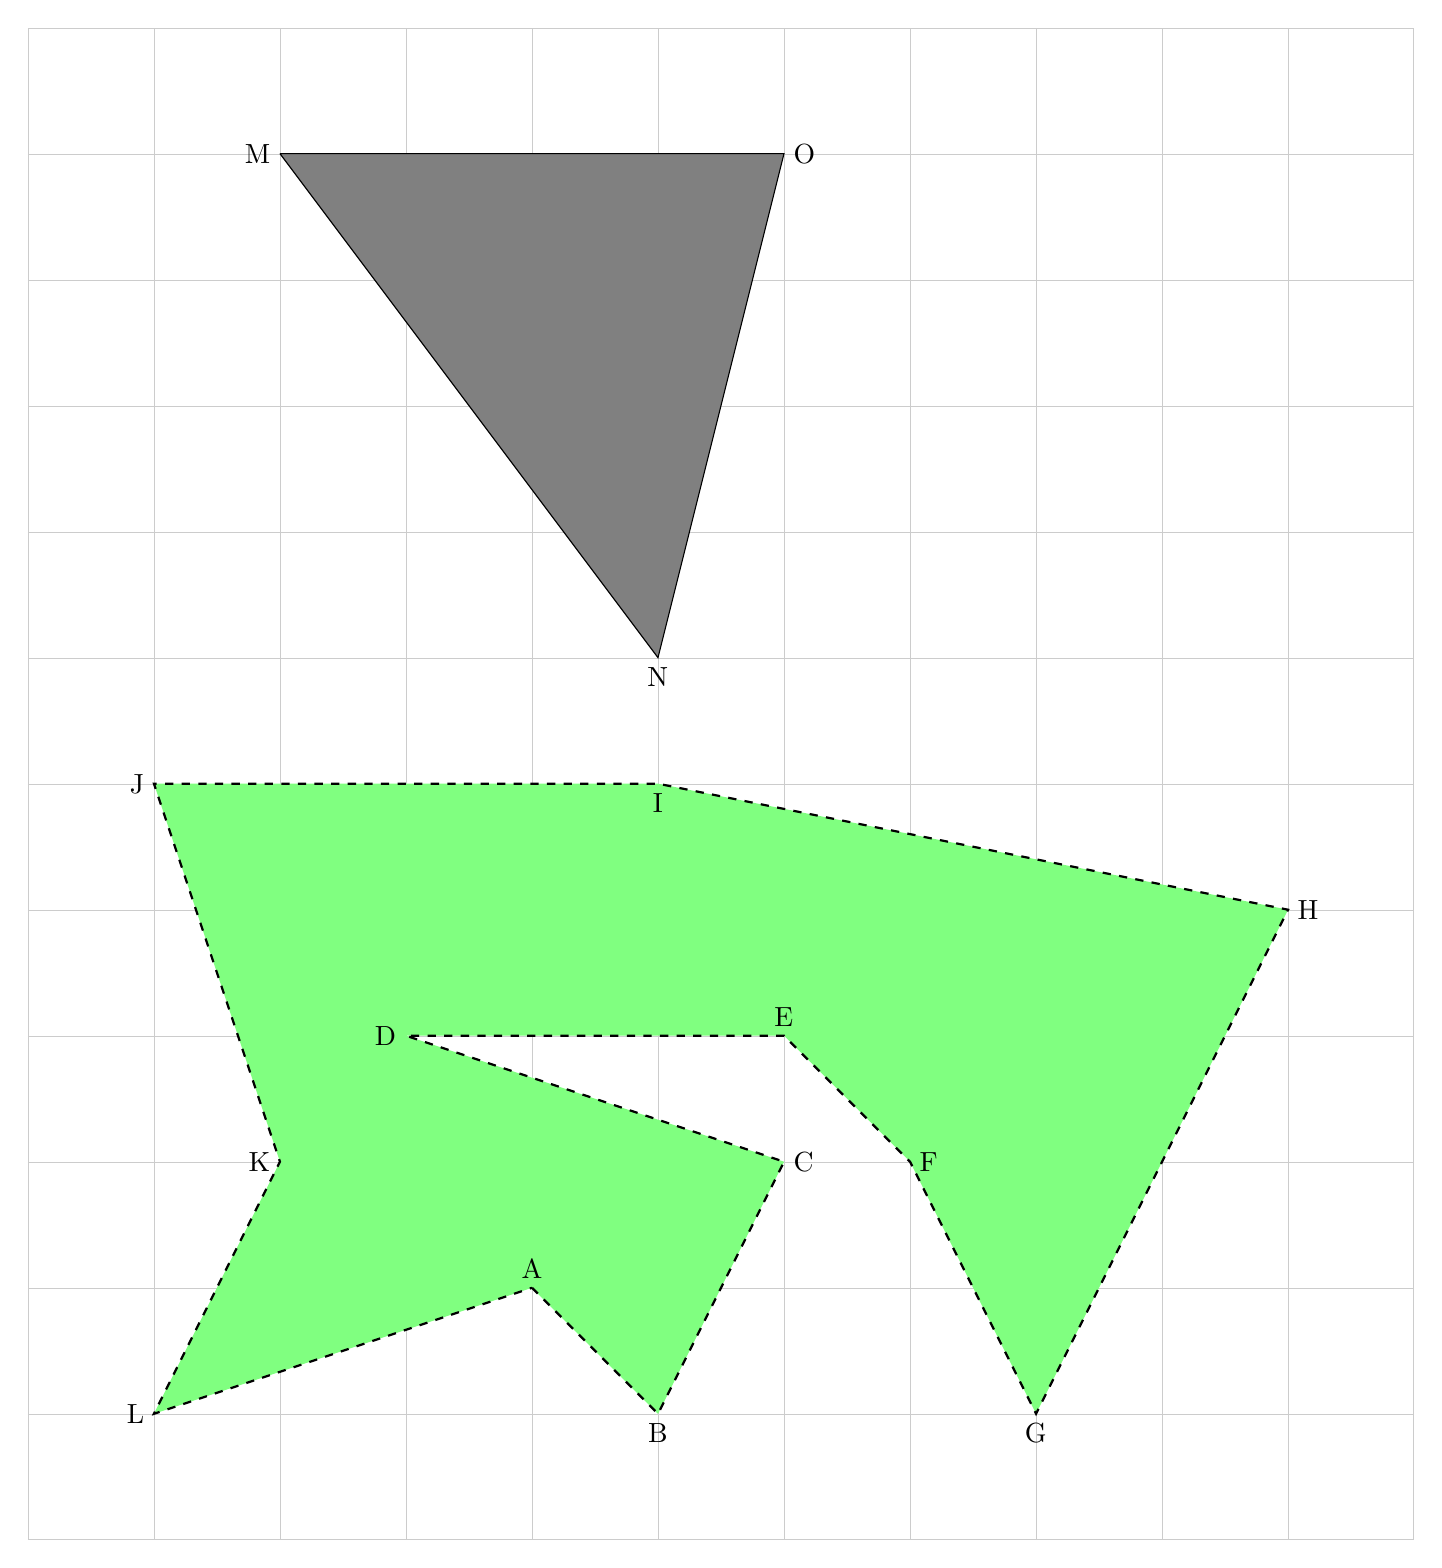
\begin{tikzpicture}[scale=1.6]

\draw [help lines, black!20] (-1,-1) grid (10,11);

\path (3,1) coordinate(A) [above] node {A};
\path (4,0) coordinate(B) [below] node {B};
\path (5,2) coordinate(C) [right] node {C};
\path (2,3) coordinate(D) [left] node {D};
\path (5,3) coordinate(E) [above] node {E};
\path (6,2) coordinate(F) [right] node {F};
\path (7,0) coordinate(G) [below] node {G};
\path (9,4) coordinate(H) [right] node {H};
\path (4,5) coordinate(I) [below] node {I};
\path (0,5) coordinate(J) [left] node {J};
\path (1,2) coordinate(K) [left] node {K};
\path (0,0) coordinate(L) [left] node {L};

\draw [fill=green!50, dashed, thick] (A)--(B)--(C)--(D)--(E)--(F)--(G)--(H)--(I)--(J)--(K)--(L)--(A);

\path (1,10) coordinate(M) [left] node {M};
\path (4,6) coordinate(N) [below] node {N};
\path (5,10) coordinate(O) [right] node {O};

\draw [fill=black!50] (M)--(N)--(O)--(M);

\path (3,1) coordinate(A) [above] node {A};
\path (2,3) coordinate(D) [left] node {D};
\path (5,3) coordinate(E) [above] node {E};
\path (6,2) coordinate(F) [right] node {F};
\path (4,5) coordinate(I) [below] node {I};

\end{tikzpicture}
\end{center}

\newpage
\begin{tikzpicture}[scale=2,xscale=1.2]
\draw [help lines, black!10] (-1,-1) grid (6,11);

\path (0,0) coordinate(A) [below] node {A};
\path (0,10) coordinate(B) [above] node {B};
\path (2,10) coordinate(C) [above] node {C};
\path (0,6) coordinate(D) [left] node {D};
\path (2,6) coordinate(E) [above] node {E};
\path (2,0) coordinate(F) [below] node {F};
\path (1,9) coordinate(G) [left] node {G};
\path (1,7) coordinate(H) [below] node {H};
\path (1,5) coordinate(I) [above] node {I};
\path (1,1) coordinate(J) [left] node {J};
\path (2,5) coordinate(K) [above] node {K};
\path (2,1) coordinate(L) [below] node {L};
\path (2,9) coordinate(M) [above] node {M};
\path (2,7) coordinate(N) [below] node {N};

\draw (F)--(A)--(B)--(C);
\draw (D)--(E);
\draw (L)--(J)--(I)--(K);
\draw (N)--(H)--(G)--(M);

\draw (C) arc (90:-90:2);
\draw (M) arc (90:-90:1);

\draw (K) arc (90:-90:2);
\draw (E) arc (90:-90:3);
\end{tikzpicture}

\end{document}